\chapter{Conclusion and discussion}
\label{chap:discussion}

\section{Summary of findings}
In language after language, we see three clause types (\diis{}) dedicated to three speech acts (\aqrs{}), and by 18 months old, children seem to be able to differentiate these clause types and associate them with their canonical speech act. To gain this ability, they need to identify the right categories of clauses (the clustering problem) and figure out what speech act they are canonically used for (the labeling problem). To solve the labeling problem, some speech act information must be available, but if there are too many mismatching cases between speech acts and clause types, this information might not be useful after all. To solve the clustering problem, children need to pay attention to the surface morpho-syntactic features of each sentence in their input. But in the input, the surface features might be absent or misleading. Again, it seems plausible that speech act information can help, but this information too is potentially misleading.

This dissertation investigates how children figure out clause type categories. In particular, are the surface formal features of the sentences in the input sufficient for children to figure out the clustering of clause types? If not, is speech act information helpful for solving the clustering problem?

I addressed these questions computationally by simulating two learners, a \distlearner{} (\dlearnerabbr{}), and a \praglearner{} (\plearnerabbr{}). Both learners use the surface morpho-syntactic features of the input sentences to attempt to cluster sentences into three categories, i.e.\ to learn the clause type categories. But the \plearnerabbr{} additionally has access to information about which speech act is performed by a sentence. I found that in English, the \dlearnerabbr{} model could identify interrogative clause but could not identify the other two clauses, but in Mandarin, this model cannot find any of the right categories. The \plearnerabbr{} model in both languages outperform the \dlearnerabbr{}. In English, the \plearnerabbr{} model can find all three clause types; in Mandarin, the model  has problem with imperative clauses. These results suggest that pragmatics is helpful, indeed crucial, to solve the clustering problem. 

But if the speech act information is useful for clause type learning, how do children figure out speech act information? Given that the way we generally identify a speech act is via its clause type, there is a potentially vicious circle here --- you need to know the clause type to identify the speech act but you need to know the speech act to identify the clause type. How do learners avoid this circularity?

One way to break this circularity is to \tit{not} think of the learning of speech acts and clause types as two processes that need to happen sequentially, but as a joint learning process. It is likely that children learn to identify speech act and clause type in tandem and mutually informative ways.

To get one step closer from this joint learning hypothesis, I first addressed the question of how much speech act information children need to identify clause types. With the \plearnerabbr{} model, I simulated the learning of clause type with various degrees of noise in the speech act information. I showed that even if children can only perceive speech act information a small proportion of the time, they can still benefit from this information, as a noisy pragmatic percept is superior to no pragmatics at all. 

I then explored what kind of non-clause type cues for speech act information is present in the input. Even if children must rely on clause type information to figure out the speech acts, they could have access to additional information that is unrelated to clause typing, but informative for recognizing speech act type. When speakers perform speech acts, because of the conventional functions of these speech acts on the discourse, the performance might be associated with certain socio-pragmatic features. For example, because of questions' response-elicitation function, we would expect pauses after questions. With prior knowledge about communication, and expectations about what questions do, children might able to use these socio-pragmatic features to figure out this speech act. If children have such expectations, would they find anything in the input? 

I explored three cues that could potentially differentiate questions from other speech acts prosody, pauses, and direct eye gaze. I found that parents do not use final rises more often with questions, but polar interrogatives have more final rises than other types of speech acts and clause types, including \twh-interrogatives and declaratives. Although due to the limitation of the pitch identification algorithm, these results are still preliminary, and we need manually annotated pitch data to draw further conclusions. Moreover, parents tend to pause longer after questions, and attend the child more when asking questions. Therefore it is in principle plausible that there are some socio-pragmatic features that children can use, in addition to their growing knowledge of clause types to infer the speech act category of an utterance. This little bit of information about speech act could then be used to provide enough pragmatic information that the child needs in order to get the clause type clusters identified accurately.

\section{The pragmatic syntactic bootstrapping hypothesis}



When examined separately, the learning of clause types and the learning of speech acts share many similarities. 
%The learning of clause types seem to parallel with the learning problems typically associated with the semantic bootstrapping hypothesis, and the learning of speech act categories seem to parallel to some degree to the problems addressed by the syntactic bootstrapping hypothesis. Let's look at them one by one. 


The clause type categories are abstract formal features of a sentence related to a variety of surface forms, none of which is obligatorily present and many of which can occur in sentences with a different clause-type feature. While in principle the surface formal features could be sufficient, this dissertation showed that they in fact fall short. To compensate for this insufficiency, learners can use the speech act information --- which systematically related to clause types --- to find the right way for clause typing.  

%Leaving aside the nature of speech act categories for now, but they are also not directly observable from the input, same as clause types, and need to be inferred. 
Speech acts are abstract pragmatic/semantic/conceptual categories. As we have seen in Chapter~\ref{chap:eng-sp}, speech act categories are related to a variety of human behaviors (e.g. pauses and eye gaze), none of which is obligatorily present (you don't need to pause after a question) and many of which can occur when performing other speech act categories. While I showed that the features are correlated with the use of questions, it is likely that the learners use the clause type information --- which systematically related to speech acts --- to constrain their inference of speech acts.  

In both learning processes, one source of information could bridge the gap between the learners' input and the abstract category they need to acquire, because of the robust correlations between clause types and speech acts across languages. 

But as I have discussed in previous chapters, when we put these two learning processes together, our first impression is that there is a chicken-and-egg problem: the learner needs speech act information to learn clause types, but they also needs clause types to learn speech act information. To break this vicious cycle, \hypos{} proposes that the learner has to learn the two in tandem:

\begin{exe}\ex\label{ex:prag-syn-hypo}
\tbf{The \hypos{}}:\\
Children learn to identify speech acts and clause types in tandem and mutually informative ways: children learn to identify clause types by tracking formal regularities in conjunction with their growing knowledge of speech acts and its associated social pragmatic cues; similarly, they identify speech acts by tracking social pragmatic cues in conjunction with their growing understanding of the syntax of clause types. 
\end{exe} 

\bex{}
\ex
\begin{tikzpicture}[level distance=60pt]
\tikzset{every tree node/.style={align=center,anchor=north, font=\scriptsize}}
%}}
\tikzset{level 1/.style={level distance=35pt}}
\tikzset{level 2/.style={sibling distance=35pt}}
%\tikzset{level 3/.style={sibling distance=-6pt}}
%\tikzset{level 4+/.style={sibling distance=-6pt}}
\Tree
[. {Sentential force} 
	[. {Clause type features\\ ([\textpm int, imp])} 
		[. {Surface formal features} ]
		[. {Prosodic features} ]
	]
	[. {Speech act categories \\
	\aqrs{}} 
		[. {Social pragmatic features} ]
		[. {Prosodic features} ]
	]
]

\end{tikzpicture}
\eex

In this dissertation, I have established that (a) the learning of clause types does not require perfect speech act information, which makes it possible that children learn clause type information while still trying to figure out the speech act information. (b) There are social pragmatic cues associated with the use of the question speech act. So if a child is armed with a theory of what questions do, in addition to an innate knowledge that there are speech act categories, they could potentially find the signals they need.

In future work, I plan to provide a proof of concept for the \hypos{} for the acquisition of questions and interrogatives.  



%%%%
\begin{comment}
Previously, \textcite{hacquardlidz2018} proposes the \hypos{} to address the learning of attitude verbs like \tit{think}. In their paper, the hypothesis is proposed for the learning of an abstract semantic property (the semantic class of an attitude verb) that is systematically related to (a) syntactic distribution and (b) pragmatic function. The \hypos{} is proposed to deal with the problem that observations of only the syntactic distribution or only the pragmatic function had the potential to mislead, so each was used to constrain the other. 

In our situation, the learners need to figure out two abstract categories, the clause types and the speech acts information, and the formulation seems to be that the two categories need to be learned in tandem.

\tbf{The \hypos{}} (alternative):\\
Children learn to identify the sentential force of a sentence by observing the speech acts that the sentence is used to perform on the one hand, and observing the syntactic clause types in tandem and mutually informative ways: children learn to identify clause types by tracking formal regularities in conjunction with their growing knowledge of speech acts and its associated social pragmatic cues; similarly, they identify speech acts by tracking social pragmatic cues in conjunction with their growing understanding of the syntax of clause types. 

because of the systematic mapping between the three major clause types and the three major speech acts, 
The semantic bootstrapping hypothesis states that:
\begin{quote}
[T]he child uses the presence of \tit{semantic} entities such as ``thing,'' ``causal agent,'' ``true in past'' and ``predicate-argument relation'' to infer that the input contains tokens of the corresponding syntactic substantive universals such as \tit{noun}, \tit{subject}, \tit{auxiliary}, \tit{dominates} and so on.\\
\hspace*{\fill} \cite[407]{pinker1987} 
\end{quote}
\end{comment}
%%%%

%When putting these two together, it first appears that we might have a chicken-and-egg problem: 

